\clearpage
\section{Odvození tržní křivky nabídky. Faktory ovlivňující nabídku. Cenová elasticita nabídky.}

\subsection{Odvození}
\begin{itemize}
    \item Postup stejný jako u tržní poptávky, vycházíme z toho, že celkové nabízené množství je 
    součtem individuálních nabízených množství jednotlivých prodejců. $Q=q_1+q_2+\dots +q_n$
    \item Převedeme z tvaru $p=a\cdot q+b$ na $q=\frac{p-b}{a}$
    \item Sečíst,  $Q=\frac{p-b_1}{a_1}+\frac{p-b_2}{a_2}+\dots +\frac{p-b_n}{a_n}$
    \item Převést na tvar $S:P=c\cdot Q + d$
    \item Nebo graficky, sčítáme jednotlivé množství
\end{itemize}
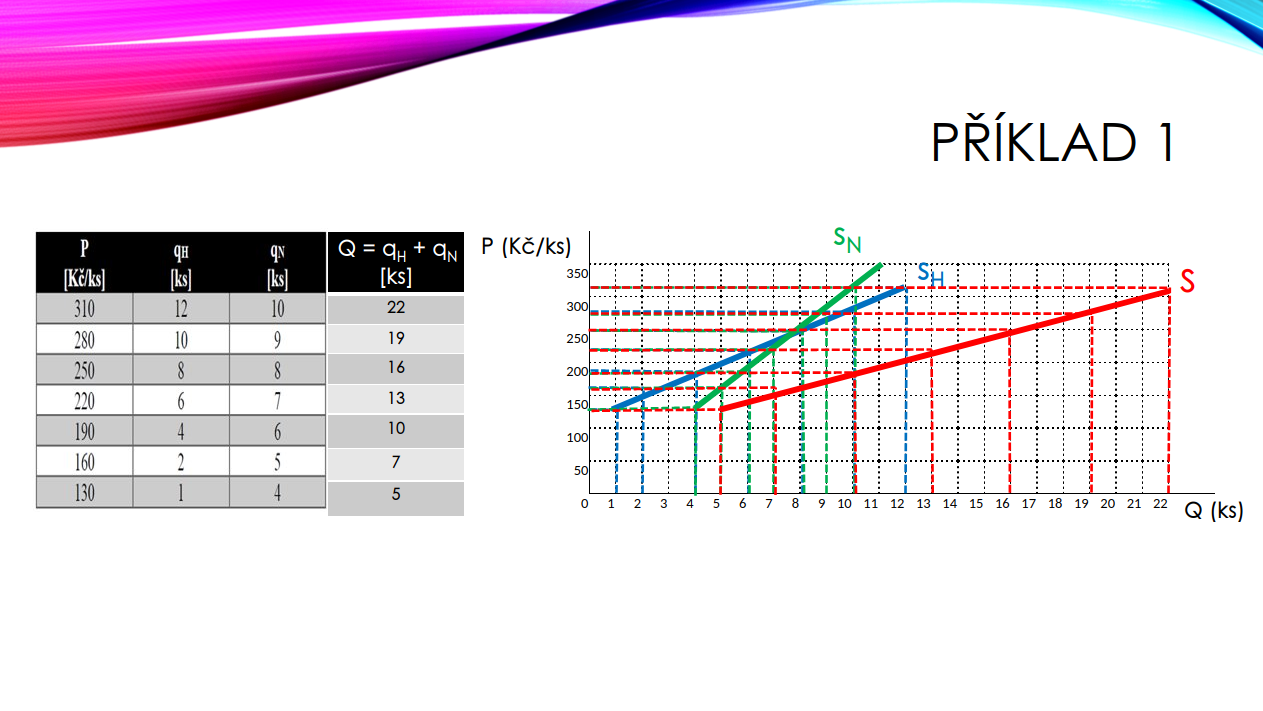
\includegraphics[width=16cm]{images/10_graficky.png}

\subsection{Faktory ovlivňující nabídku}
\begin{enumerate}
    \item Cenové faktory (posun po nabídkové křivce)
    \begin{itemize}
        \item Změna ceny
    \end{itemize}
    \item Necenové faktory (posun nabídkové křivky)
    \begin{itemize}
        \item Dokonalost technologií
        \item Očekávaná změna ceny
        \item Vstup nového prodejce na trh
        \item Změna ceny surovin
    \end{itemize}
\end{enumerate}

\subsection{Cenová elasticita}
\begin{itemize}
    \item $E_{PS}=\frac{\% \Delta Q_S}{\% \Delta P_S}$, kde $Q$ je množství a $P$ je cena
    \item Obdobně jako u poptávky
\end{itemize}